\begin{framed}

Objetivos:
\begin{itemize}
    \item Encontrar la relación entre variables termodinámicas de un flujo isentrópico de un gas ideal y sus condiciones de estancamiento.
    \item Estudiar la forma de obtener un flujo supersónico desde una tobera.
    \item Describir el flujo compresible en una tobera convergente-divergente.
\end{itemize}

Contenidos:
\begin{itemize}
    \item Flujo isentrópico de gas ideal y sus condiciones al estancamiento. 
    \item Flujo en una tobera convergente y divergente en el caso subsónico y supersónico. 
    \item Condiciones críticas y flujo ahogado.
    \item La tobera convergente-divergente.
\end{itemize}

Bibliografía:
\begin{itemize}
    \item Fox, R. W., Pritchard, P. J. y McDonald, A. T. (2009) Introduction to Fluid Mechanics. John Wiley \& Sons. Sección 12.3-13.2.
\end{itemize}
\end{framed}

\section*{Flujo isentrópico de un gas ideal}
\subsection*{Relaciones termodinámicas con el estancamiento}

En la clase pasada repasamos conceptos de termodinámica, y llegamos a diferentes expresiones relacionando presión, temperatura y densidad para procesos isentrópicos de gases ideales. 
Ahora, analizaremos un flujo isentrópico de gas ideal, para poder encontrar ecuaciones que relacionen un estado termodinámico con las condiciones del flujo al estancamiento.
Poder saber las condiciones termodinámicas de un flujo respecto a su estado de estancamiento es de gran utilidad para aplicaciones, ya que conociendo las condiciones del gas en un estanque (donde está quieto), podemos predecir su estado, por ejemplo, a lo largo de una tobera.

Analicemos un flujo isentrópico de un gas ideal que va desacelerándose hasta llegar a velocidad 0 (estancamiento), usando un tubo de corriente de ancho $dx$ como volumen de control (Figura \ref{fig:volumen_control}).
%
\begin{figure}
\centering
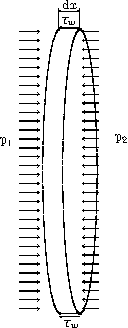
\includegraphics[width=0.7\textwidth]{clase14/volumen_control.pdf}
\caption{Volumen de control sobre línea de corriente que llega a la condición de estancamiento}
\label{fig:volumen_control}
\end{figure}
%
El volumen de control se encuentra en un punto genérico $x$, donde la velocidad del flujo es $V$, densidad $\rho$, presión $p$, temperatura $T$ y el tubo de corriente tiene area $A$. 
Después del volumen de control, estas condiciones cambian a $V+dV$, $\rho+d\rho$, $p+dp$, $T+dT$ y $A+dA$.
Aguas abajo, el flujo de desacelera a velocidad $V=0$, y encontramos las condiciones de estancamiento $\rho_0$, $p_0$ y $T_0$.

Partamos por analizar continuidad sobre el volumen de control.
Ya que es un tubo de corriente, no hay flujo a través del ``manto'' del volumen de control, si no que solamente por las secciones transversales.
Digamos que la velocidad y densidad son constantes en cada sección transversal (lo cual no es una mala aproximación si consideramos un $A$ pequeño).
En estado estacionario (sin acumulación), la conservación de masa nos lleva a
%
\begin{equation}\label{eq:continuidad_isentropico}
\rho VA = (\rho+d\rho)(V+dV)(A+dA)
\end{equation}

El análisis de cantidad de movimiento es un poco más engorroso.
De Mecánica de Fluidos General, sabemos que si no hay acumulación, el teorema de transporte de Reynolds en conjunto con la segunda ley de Newton da:
%
\begin{equation}\label{eq:momentum_isentropico}
\sum \mathbf{F} = \oint_S \mathbf{V} \rho \mathbf{V}\cdot\mathbf{n} dS.
\end{equation}

Partamos con la suma de fuerzas en el eje $x$.
Usando la Figura \ref{fig:cantidad_mov} como referencia, en las caras transversales tenemos una fuerza $pA$ por el lado izquierdo y $(p+dp)(A+dA)$ por el derecho.
Por otra parte, el manto tiene una forma arbitraria, y una distribución de presión sobre ésta tiene una componente en el eje $x$.
Considerando que $dx$ es pequeño, asumamos que la presión media sobre este manto es igual al promedio lineal de la presión antes y después del volumen de control, es decir $\overline{p} = p+dp/2$.
Entonces, la fuerza sobre el manto es $(p+dp/2)S$, donde $S$ es el área del manto, y $S=Ld$ donde $L$ es el perímetro y $d$ el ancho ($dx=d\cos\alpha$) .
Nosotros estamos interesados en la componente $x$ de la fuerza, que es $(p+dp/2)Ld\sin\alpha$, pero $d\sin\alpha$ es la proyección de $d$ en el eje $y$, y multiplicado por el perímetro $L$, no es más de la diferencia entre las áreas de entrada y salida del volumen de control ($dA$).
De esta forma, podemos escribir la componente $x$ de la fuerza sobre el manto como $(p+dp/2)dA$, y despreciando los términos con diferenciales de orden mayor a 1, la suma de fuerza queda
%
\begin{equation}
\sum F_x = pA - (p+dp)(A+dA) + (p+dp/2)dA = -dpA
\end{equation}
%
\begin{figure}
\centering
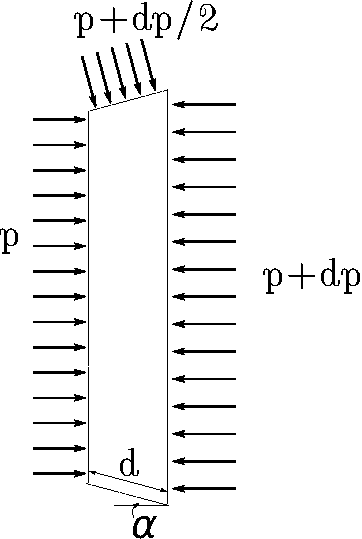
\includegraphics[width=0.3\textwidth]{clase14/cantidad_mov.pdf}
\caption{Análisis de cantidad de movimiento sobre volumen de control.}
\label{fig:cantidad_mov}
\end{figure}

Conociendo la suma de fueras, y asumiendo que la variables son constantes en la sección transversal, podemos reescribir la Ec. \eqref{eq:momentum_isentropico} como
%
\begin{align}\label{eq:momentum_isen_final}
-dpA &= -V\rho VA + (V+dV)\underbrace{(\rho+d\rho)(V+dV)(A+dA)}_{=\rho VA\text{ por continuidad (Ec.\eqref{eq:continuidad_isentropico})}}\nonumber\\
\Rightarrow -dp &= \rho V(-V+V+dV)\nonumber\\
-dp &= \rho VdV\nonumber\\
\frac{dp}{\rho} &+ d\left(\frac{V^2}{2}\right) = 0
\end{align}

Hasta ahora, nada hemos dicho de gases ideales ni de flujo isentrópico; utilicemos estos conceptos.
De la clase pasada, sabemos que para un flujo isetrópico ideal
%
\begin{equation}\label{eq:isentropico}
\frac{p}{\rho^k} = C_0,
\end{equation}
%
por lo que podemos reescribir la Ec. \eqref{eq:momentum_isen_final} como
%
\begin{equation}
-C_0^{1/k}\frac{dp}{p^{1/k}} = d\left(\frac{V^2}{2}\right).
\end{equation}
%
Integremos esta última expresión desde $x$ hasta el punto de estancamiento
%
\begin{align}\label{eq:p_isen}
-\int_V^0d\left(\frac{V^2}{2}\right) &= C_0^{1/k}\int_p^{p_0}p^{-1/k}dp\nonumber\\
\frac{V^2}{2} = C_0^{1/k} \left.\frac{1}{1-\frac{1}{k}}p^{1-1/k}\right/_p^{p_0}&= C_0^{1/k}\left.\frac{k}{k-1}p^{\frac{k-1}{k}}\right/_p^{p_0}\nonumber\\
=C_0^{1/k}\frac{k}{k-1}\left(p_0^{\frac{k-1}{k}}-p^{\frac{k-1}{k}}\right) &= C_0^{1/k}p^{\frac{k-1}{k}}\left[\left(\frac{p_o}{p}\right)^{\frac{k-1}{k}}-1\right]\nonumber\\
\text{ pero de la Ec. \eqref{eq:isentropico}:   } C_0^{1/k} &= \frac{p^{1/k}}{\rho}\nonumber\\
\Rightarrow\frac{V^2}{2}&=\frac{k}{k-1}\frac{p}{\rho}\left[\left(\frac{p_o}{p}\right)^{\frac{k-1}{k}}-1\right]\nonumber\\
\text{despejando...   } \frac{p_0}{p} &= \left[\frac{V^2}{2}\frac{k-1}{k}\frac{\rho}{p}+1\right]^\frac{k}{k-1}\nonumber\\
\text{y usando la ley de gases ideales   } \frac{p_0}{p} &= \left[\frac{V^2}{2}\underbrace{\frac{k-1}{k}\frac{1}{RT}}_{kRT=c^2}+1\right]^\frac{k}{k-1}\nonumber\\
\Rightarrow \frac{p_0}{p} &= \left[M^2\frac{k-1}{2}+1\right]^\frac{k}{k-1}
\end{align}

A partir de la Ec. \eqref{eq:isentropico}, podemos escribir
%
\begin{equation}
\frac{p}{\rho^k} = \frac{p_0}{\rho_0^k} \Rightarrow \frac{p_0}{p} = \left(\frac{\rho_0}{\rho}\right)^k,
\end{equation}
%
y usando la Ec. \eqref{eq:p_isen}, llegamos a
%
\begin{equation}\label{eq:rho_isen}
\frac{\rho_0}{\rho} = \left(\frac{p_0}{p}\right)^{1/k} = \left[M^2\frac{k-1}{2}+1\right]^\frac{1}{k-1}.
\end{equation}
%
Por otra parte, desde la ley de gases ideales podemos decir que
%
\begin{align}\label{eq:T_isen}
\frac{P}{\rho}&=RT \quad \frac{p_0}{\rho_0} = RT_0\Rightarrow \frac{T_0}{T} = \frac{p_0}{p}\frac{\rho}{\rho_0}\nonumber\\
\Rightarrow \frac{T_0}{T} &= \left[M^2\frac{k-1}{2}+1\right]^{\frac{k}{k-1}-\frac{1}{k-1}} = M^2\frac{k-1}{2}+1.
\end{align}

Lo interesante de todas estar relaciones es que solamente dependen del número de Mach. 
Por lo tanto, dado un gas que está quieto en un estanque a $p_0$, $\rho_0$ y $T_0$, si se mueve de forma isentrópica, las condiciones termodinámicas están definidas únicamente por su velocidad.
Existen tablas de flujo isentrópico que no son más que la solución de las Ecs. \eqref{eq:p_isen}, \eqref{eq:rho_isen} y \eqref{eq:T_isen} para diferentes números de Mach.

\subsection*{Flujo en un ducto de área variable}

Digamos que tenemos un flujo compresible dentro de un ducto de área variable, como el de la Figura \ref{fig:tobera}. 
Por continuidad sabemos que el flujo másico es constante a lo largo del ducto, y diferenciando:
%
\begin{align}\label{eq:d_mpunto}
&\left.\dot{m}=\rho V A\right/ d,\nonumber\\
&\left.0 = d\rho VA + \rho dV A + \rho V dA\right/\cdot\frac{1}{\rho VA}, \nonumber\\
&0 = \frac{d\rho}{\rho} + \frac{dV}{V} + \frac{dA}{A}  
\end{align}

\begin{figure}
\centering
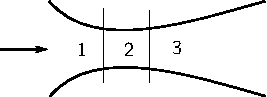
\includegraphics[width=0.5\textwidth]{clase14/tobera.pdf}
\caption{Flujo en ducto de área variable. La región $1$ es convergente, la región $2$ aproximadamente recta y la sección $3$ divergente.}
\label{fig:tobera}
\end{figure}

Miremos nuevamente la Ec. \eqref{eq:momentum_isen_final}, y reescribámosla como
%
\begin{align}\label{eq:momentum_isen_aux}
&\left.\frac{dp}{\rho} + VdV = 0\right/\cdot\frac{1}{V^2}\nonumber\\
&\Rightarrow\frac{dp}{\rho V^2} = -\frac{dV}{V}
\end{align}
%
y usemos este último resultado en la Ec. \eqref{eq:d_mpunto}:
%
\begin{align}
\frac{dA}{A} &= \frac{dp}{\rho V^2} - \frac{d\rho}{\rho} = \frac{dp}{\rho V^2} \Big[1-\underbrace{\frac{d\rho}{dp}}_{=1/c^2} V^2\Big]\nonumber\\
&=\frac{dp}{\rho V^2} \left[ 1-\frac{V^2}{c^2}\right] = \frac{dp}{\rho V^2}\left[1-M^2\right].
\end{align}
%
Nuevamente, usemos la Ec. \eqref{eq:momentum_isen_aux} para escribir
%
\begin{align}\label{eq:tobera}
\frac{dA}{A} &= -\frac{dV}{V}\left[1-M^2\right]\nonumber\\
\Rightarrow \frac{dV}{V}&=-\frac{dA}{A}\frac{1}{1-M^2}
\end{align}

Esta última ecuación nos dice cosas muy interesantes, y que a primera vista, son poco intuitivas.
Lo primero es el significado físico de los diferenciales: $dV$ no es más que la variación de velocidad a lo largo de ducto, y $dA$ la variación de área; veamos su relación en diferentes casos.
%
\paragraph*{Caso subsónico ($M<1$).} Reemplazando $M$ en la Ec. \eqref{eq:tobera}, nos queda una expresión negativa al lado derecho, por ende, una relación inversa entre $dA$ y $dV$.
Esto implica que si uno crece el otro se achica, por ejemplo, al disminuír el área, crece la velocidad.
Este es el comportamiento que esperamos, considerando nuestros conocimientos previos de mecánica de fluidos.
En el contexto del ducto de la Figura \ref{fig:tobera}, el flujo se acelera en la zona $1$ y se frena en la zona $3$.
%
\paragraph*{Caso supersónico ($M>1$):} Acá la cosa cambia un poco. Al ser $M>1$, el denominador al lado derecho pasa a ser negativo, y cancela el signo menos al frente de la expresión, por lo que $dA$ tiene una relación directa con $dV$.
En términos físicos, esto significa que si se achica el área, se frena el flujo: ¡Totalmente lo contrario respecto al caso subsónico (y lo que dice nuestra intuición)!
Entonces, de ser supersónico, el flujo de frenaría en la zona $1$ de la Figura \ref{fig:tobera}, y se acelera cuando está en la zona $3$.
%
\paragraph*{Caso sónico ($M=1$):} Ahora si que estamos en problemas, ya que la Ec. \eqref{eq:tobera} se indefine.
Físicamente esto no tiene sentido, y el sistema se debiese ajustar a esta situación.
La única forma que no se indefina es que $dA=0$: solamente tendremos la velocidad del sonido dentro de un ducto cuando no hay variación de área, como en la región $2$ de la Figura \ref{fig:tobera}.

\mbox{?`}Qué ocurre físicamente que el caso supersónico es tan poco intuitivo?
Para encontrar una respuesta, hay que mirar la Ec. \eqref{eq:d_mpunto}, que reacomodamos de la siguiente forma:
%
\begin{equation}
\frac{dV}{V} = -\frac{d\rho}{\rho} - \frac{dA}{A},
\end{equation}
%
indicándonos que la variación de velocidad es un balance entre la variación de área y la variación de densidad.
Resulta que para el caso supersónico los efectos de densidad se hacen más importantes que los de área.
Por ejemplo, en una zona convergente, la disminución de área produce un aumento de densidad tal que $d\rho/\rho$ domina sobre $dA/A$, frenando el flujo.
Lo contrario en la zona divergente, donde el aumento de área produce una baja de densidad tal que se acelera el flujo.

\section*{Flujo ahogado}

Digamos que tenemos la tobera convergente de la Figura \ref{fig:tobera_convergente}.
La tobera tiene una salida recta, que llamamos garganta, de forma que es posible que la descarga sea a $M=1$ según las condiciones en $dA$ que discutimos antes. 
Por otra parte, el estanque de entrada tiene una presión $p_0$, mientras que el de salida tiene $p_s$, y en este ejercicio simulado vamos a suponer que bajamos $p_s$ para lograr el flujo deseado.
Consideramos la $p_0$ como la presión de estancamiento en vez de $p_s$ porque para lograr $p_s$ en el estanque de salida debemos poner un dispositivo (compresor, soplador, etc.) que saque el gas y baje la presión, por lo que el gas no se detiene realmente en el estanque de salida. 
En el estanque de entrada, podemos considerar que lejos de la boquilla la velocidad es efectivamente cero.
%
\begin{figure}
\centering
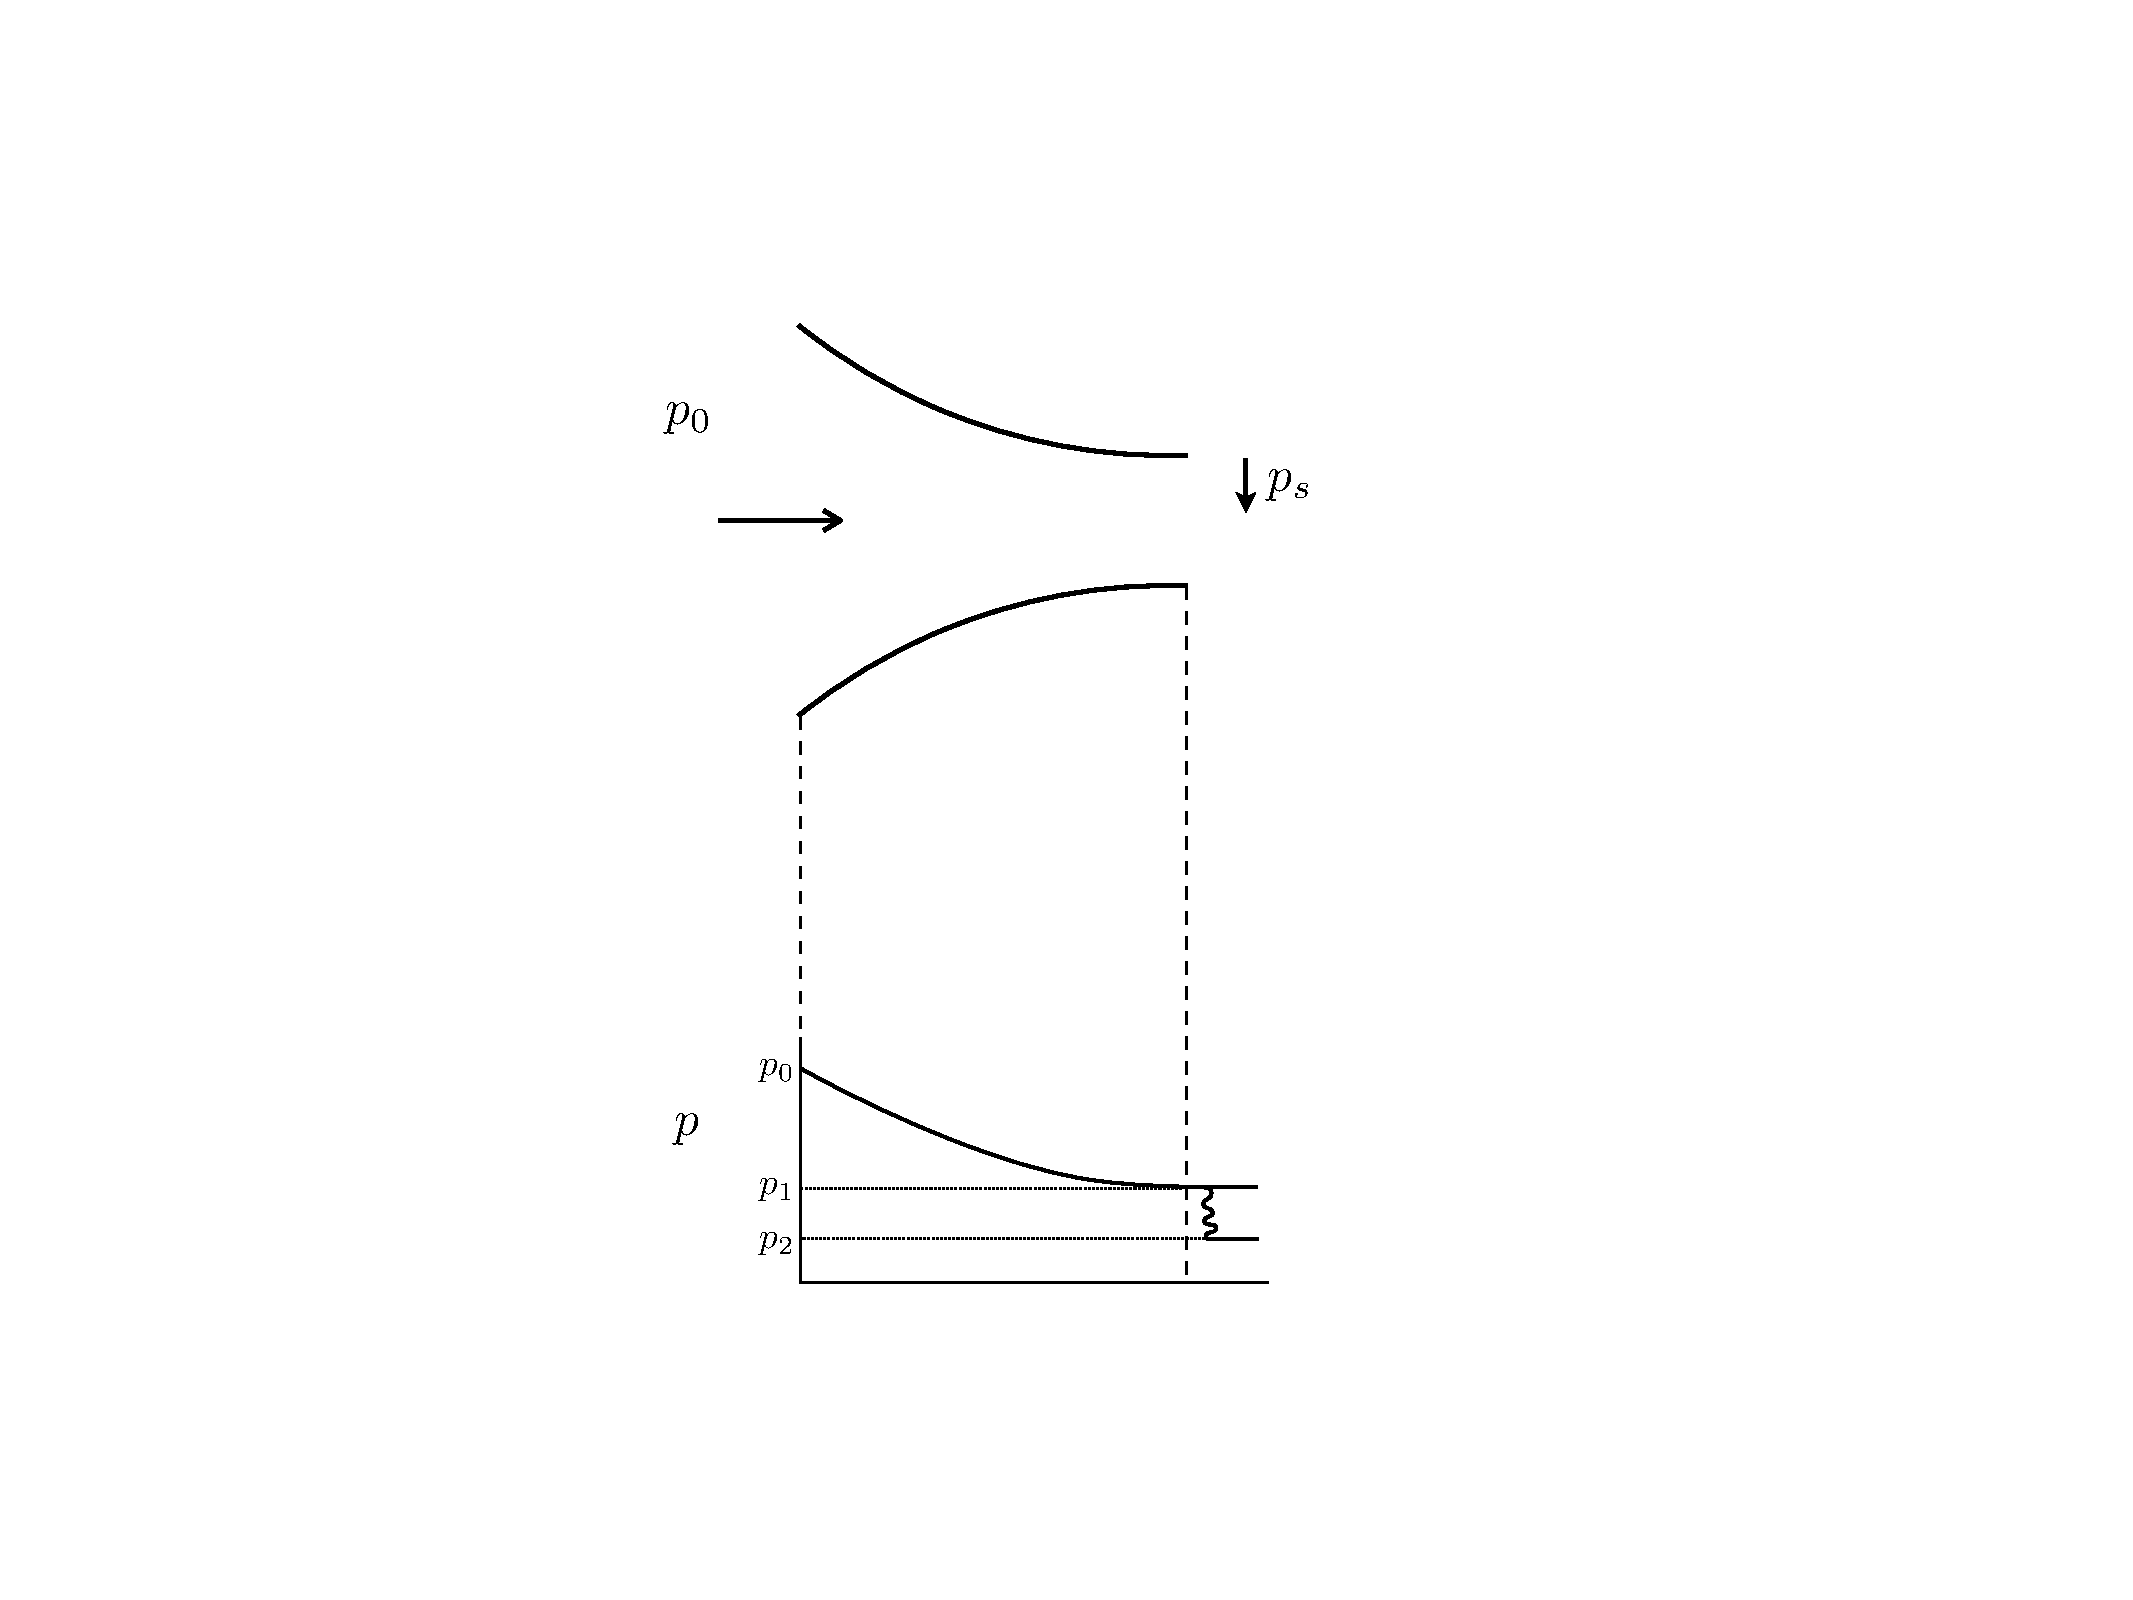
\includegraphics[width=0.4\textwidth]{clase14/tobera_convergente.pdf}
\caption{Tobera convergente. La presión $p_1$ es la presión del estanque a la salida para lograr $M=1$ en la boquilla.}
\label{fig:tobera_convergente}
\end{figure}

Bajamos entonces la presión $p_s$ hasta que $p_s=p_1$, logrando así $M=1$ en la descarga, y obtenemos la distribución de presión de la Figura \ref{fig:tobera_convergente} dentro de la boquilla.
Las condiciones cuando $M=1$ se denominan condiciones críticas, y se denotan como $p^*$, $\rho^*$, $A^*$, $V^*$ y $T^*$.
Si logramos la condición crítica en la garganta, decimos que el flujo está ``ahogado''.

El área crítica $A^*$ se usa como referencia para presentar el área en la sección transversal de la boquilla.
Para llegar a esta expresión, usamos el principio de continuidad:
%
\begin{align}
\rho VA &= \rho^* V^* A^*\nonumber\\
\Rightarrow \frac{A}{A^*} &= \frac{\rho^* V^*}{\rho V} = \frac{\rho^* c^*}{\rho Mc} = \frac{\rho^*}{\rho} \frac{1}{M}\frac{\sqrt{kRT^*}}{\sqrt{kRT}}\nonumber\\
&=\frac{\rho^*/\rho_0}{\rho/\rho_0} \frac{1}{M}\frac{\sqrt{T^*/T_0}}{\sqrt{T/T_0}}.
\end{align}
%
Usando las Ecs. \eqref{eq:rho_isen} y \eqref{eq:T_isen}, y sabiendo que $M=1$ en las condiciones críticas, llegamos a
%
\begin{equation}
\frac{A}{A^*} = \frac{1}{M} \frac{\left[\frac{k+1}{2}\right]^{-\frac{1}{k-1}}}{\left[\frac{k-1}{2}M^2+1\right]^{-\frac{1}{k-1}}} \sqrt{\frac{\frac{k-1}{2}M^2+1}{\frac{k+1}{2}}} = \frac{1}{M} \left[\frac{1+\frac{k-1}{2}M^2}{\frac{k+1}{2}}\right]^{\frac{k+1}{2(k-1)}}.
\end{equation}
%
Además, podemos calcular la presión de salida ($p_1$) necesaria para obtener $M=1$ en la garganta reemplazando $M=1$ en la Ec. \eqref{eq:p_isen}, lo que nos da
%
\begin{equation}\label{eq:p_critico}
\frac{p_1}{p_0} = \frac{p^*}{p_0} = \left(\frac{2}{k+1}\right)^{\frac{k}{k-1}}.
\end{equation}

Por otra parte, el flujo másico para el flujo ahogado es
%
\begin{align}\label{eq:mpunto_ahogado_aux}
\dot{m}_\text{ahogado} &= \rho^* V^*A^* = \frac{p^*}{RT^*}c^*A^*\nonumber\\
&= \frac{p^*}{RT^*}\sqrt{kRT^*}A^* = \frac{p^*}{\sqrt{T^*}}\sqrt{\frac{k}{R}}A^*.
\end{align}
%
Viendo la Ec. \eqref{eq:p_critico}, y que la temperatura crítica es
%
\begin{equation}
\frac{T^*}{T_0} = \frac{2}{k+1},
\end{equation}
%
podemos reescribir la Ec. \eqref{eq:mpunto_ahogado_aux} como
%
\begin{align}\label{eq:mpunto_ahogado}
\dot{m}_\text{ahogado} &= \left[\frac{2}{k+1}\right]^{\frac{k}{k+1}}p_0\sqrt{\frac{k+1}{2}}\frac{1}{\sqrt{T_0}}\sqrt{\frac{k}{R}}A^*\nonumber\\
\dot{m}_\text{ahogado} &= \sqrt{\frac{k}{RT_0}}\left(\frac{2}{k+1}\right)^{\frac{k+1}{2(k-1)}}p_0A^*
\end{align}

Digamos que en el ejemplo de la Figura \ref{fig:tobera_convergente} bajamos la presión de salida aún más, a $p_2$.
Intuitivamente uno pensaría que el flujo másico debiese seguir aumentando con la diferencia de presión, sin embargo, esto no es lo que ocurre.
Al bajar la presión, se genera una onda de presión que, para un flujo subsónico, viaja aguas arriba con velocidad $c$, lo que ajusta el flujo a las nuevas condiciones.
Pero en este caso el flujo es supersónico, por lo que la onda de presión más lenta que la velocidad, y es arrastrada aguas abajo.
Por esto, el flujo dentro de la tobera es ``sordo'' a lo que ocurre aguas abajo cuando $M=1$ en la garganta, limitando el flujo másico máximo a $\dot{m}_\text{ahogado}$.
Cuando la presión de salida es menor a $p^*$, el flujo sale de la tobera sin saber que la presión de descarga es aún más baja, lo que genera una \emph{onda de expansión}, equilibrando la presión del flujo a la del recipiente de salida.

\section*{Tobera convergente-divergente}

Ya vimos que para acelerar un flujo supersónico es necesario que el ducto sea divergente.
Por lo tanto, para lograr $M>1$, la tobera debe tener una forma similar a la Figura \ref{fig:tobera}, donde es subsónico en la zona $1$, alcanza $M=1$ en la garganta (zona $2$), y es supersónico en la zona $3$.

Usemos la Figura \ref{fig:tobera_cv} para hacer un experimento simulado, como en la sección anterior con la tobera convergente.
%
\begin{figure}
\centering
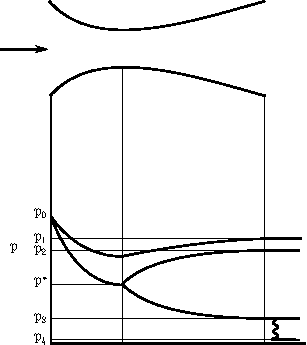
\includegraphics[width=0.5\textwidth]{clase14/tobera_cv.pdf}
\caption{Tobera convergente divergente con la distribución de presión.}
\label{fig:tobera_cv}
\end{figure}
%
Tenemos un estanque con presión $p_0$ que contiene un gas que sale por la tobera hacia un estanque con presión $p_s$, la cual podemos bajar.
Inicialmente, bajamos la presión de salida a $p_1$, pero esta presión no es suficientemente baja como para lograr flujo supersónico en la garganta.
Bajamos aún más la presión a $p_s=p_2$ y logramos las condiciones críticas en la garganta ($M=1$, $p^*$), sin embargo esta presión no es suficientemente baja como para sostener el flujo supersónico y se comporta como subsónico después de la garganta.
Si bajamos la presión aún más ($p_s=p_3$), el flujo supersónico será capaz de sostenerse a lo largo de toda la tobera, y $M>1$ a la salida.
Esta sería la condición de diseño de la tobera.
Así como en el caso convergente de la Figura \ref{fig:tobera_convergente}, al ser supersónico el flujo de salida, si bajamos la presión aún más (a $p_4$), esta información no será capaz de viajar aguas arriba (flujo dentro de la tobera es ``sordo'' a lo que ocurre aguas abajo) y se produce una onda de expansión.

Una pregunta que puede aparecer es \mbox{?`}qué pasa si la presión de salida está entre $P_2$ y $p_3$?
El flujo será supersónico, pero este régimen no podrá ser sostenido a lo largo de toda la tobera.
En este caso, en alguna parte de la zona divergente de la tobera habrá una onda de choque, que hará pasar al flujo de supersónico a subsónico, y la descarga será a $M<1$.
Vamos a hablar con más detalles de esto la próxima clase.
